\documentclass[11pt]{article}
\usepackage[margin=1in]{geometry}
\usepackage{amsmath,amssymb}
\usepackage{microtype, graphicx}

\title{A Qubit from Two Compound SIC Fiducials}
\author{}
\date{}

\begin{document}
\maketitle

The notebook \texttt{CompoundSICQubitViz.ipynb} considers the qubit
spanned by the two vectors \texttt{sachin[0][0]} and
\texttt{sachin[1][0]}, and visualizes the stabilizer entropy and LTP deformation across the Bloch sphere.
\begin{center}
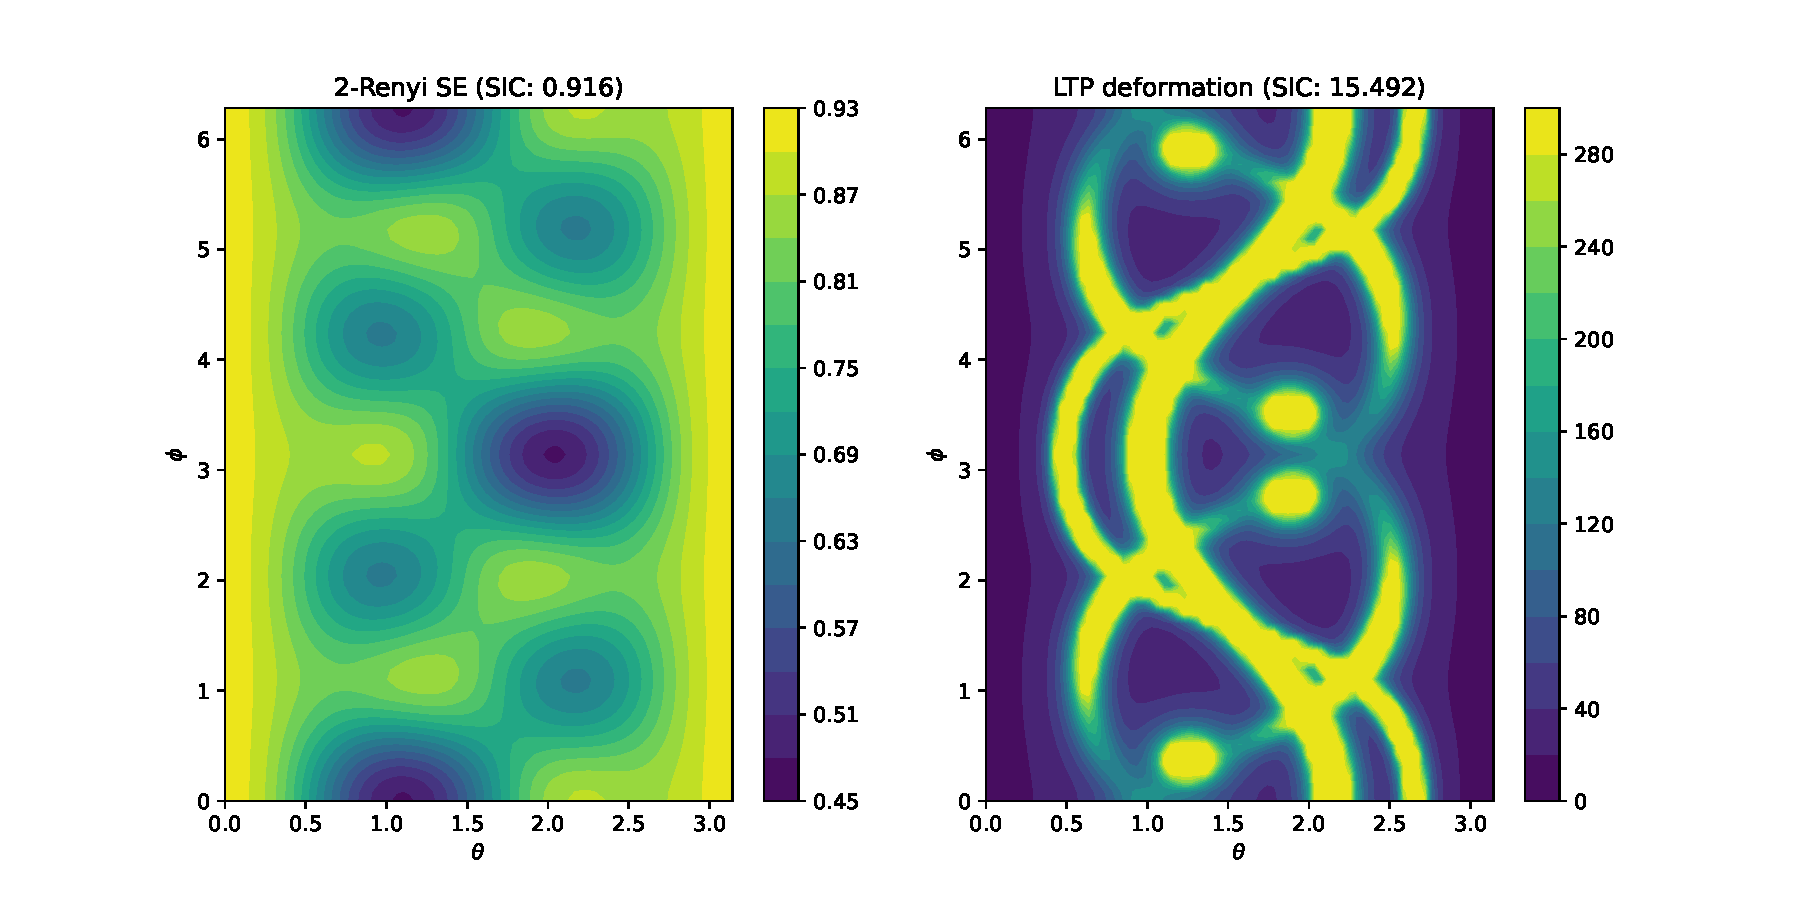
\includegraphics[scale=0.5]{compound_plot.pdf}
\end{center}
Here we give an explicit expression for its pure
states. Letting
\begin{equation}
 a=\sqrt{2+\sqrt{5}},\qquad
 b=\sqrt{\frac{1-1/\sqrt{5}}{8}},\qquad
 q=e^{i\pi/4}=\frac{1+i}{\sqrt{2}},
\end{equation}
we have for the two chosen SIC fiducials,
\begin{equation}
 |f_0\rangle=b
 \begin{pmatrix}
 1+q\\ i(1+aq)\\ q-1\\ i(1-aq)
 \end{pmatrix},
 \qquad
 |f_1\rangle=b
 \begin{pmatrix}
 -a-q\\ i(1+q)\\ a-q\\ i(1-q)
 \end{pmatrix}.
\end{equation}
These are orthonormal. Indeed, using $|q|=1$ and
$q+q^*=\sqrt{2}$,
\begin{align}
 \langle f_0|f_0\rangle
 &=\langle f_1|f_1\rangle
 =b^2(6+2a^2)=1,\\
 \langle f_0|f_1\rangle&=0.
\end{align}
Thus the general pure state of this encoded qubit is
\begin{equation}
 |\psi(\theta,\phi)\rangle
 =\cos\frac{\theta}{2}\,|f_0\rangle
 +e^{i\phi}\sin\frac{\theta}{2}\,|f_1\rangle,
 \qquad 0\leq\theta\leq\pi,\quad 0\leq\phi<2\pi.
\end{equation}
Writing $c=\cos(\theta/2)$ and $s=\sin(\theta/2)$, this becomes
\begin{equation}
 \boxed{
 |\psi(\theta,\phi)\rangle=b
 \begin{pmatrix}
 (1+q)c-(a+q)e^{i\phi}s\\[3pt]
 i\big[(1+aq)c+(1+q)e^{i\phi}s\big]\\[3pt]
 (q-1)c+(a-q)e^{i\phi}s\\[3pt]
 i\big[(1-aq)c+(1-q)e^{i\phi}s\big]
 \end{pmatrix}.}
\end{equation}
\end{document}
